\chapter{Implementation} \label{chp:implementation}

The whole project is split into two git repositories hosted at GitHub. The first repository\footnotehref{https://github.com/zouharvi/ptakopet}{github.com/zouharvi/ptakopet} contains the code for frontend, experiment data as well as some miscellaneous files regarding the whole project. The second one\footnotehref{https://github.com/zouharvi/ptakopet-server}{github.com/zouharvi/ptakopet-server} is focused strictly on the server, which is not the main focus of this thesis but is also described for completeness.

In this chapter we first describe the frontend, then the experiment architecture from a technical perspective (the experiment itself is the focus of \cref{chp:experiment}) and then the backend. See documentation in \cref{chp:development_doc} which describes all the implementation details as well as guides on how to build and setup the whole project.

\section{Frontend}
\label{sec:implementation:frontend_structure}

The web frontend is written in TypeScript because of the great scalability properties. DOM manipulation is done mostly with jQuery and the output is packed into one JavaScript file using Webpack. Packages are managed with npm (usually contained in the NodeJS package).

\begin{figure}[ht]
    \centering
    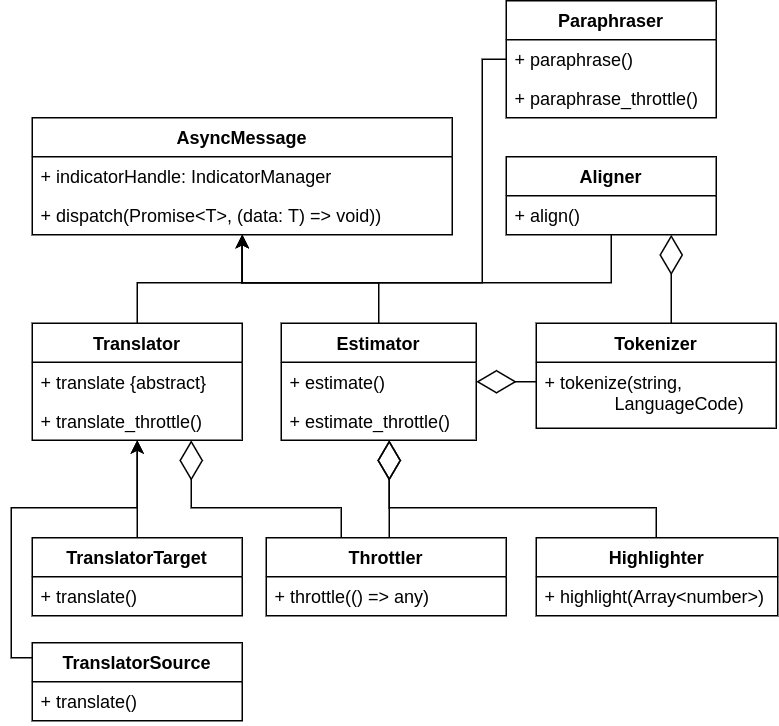
\includegraphics[width=\textwidth]{img/implementation/frontend.png}
    \caption{Object diagram of main component of the \ptakopet{} frontend}
    \label{fig:frontend_class}
\end{figure}

The diagram in \cref{fig:frontend_class} shows the overall object structure of the most important objects. These objects are: \texttt{AsyncMessage}, \texttt{Translator} (and its derivatives), \texttt{Estimator}, \texttt{Aligner}, \texttt{Paraphraser}, \texttt{Tokenizer}, \texttt{Highlighter} and \texttt{Throttler}. 

The task of \texttt{TranslatorSource} (and similarly for \texttt{TranslatorTarget}) is to translate the source sentence. Then \texttt{Estimator} has to assign word-level quality estimation scores for each target token. Finally, a word-level alignment must be computed in \texttt{Aligner}. At the end, the QE is rendered using \texttt{Highlighter}. Parallel to that, \texttt{Paraphraser} produces paraphrases for the source input and displays them.

Each of these computations could take place in the browser\footnote{This one of the goals of the Bergamot project. \href{https://browser.mt/}{browser.mt}} (\ptakopet{} includes some such mock-up solutions, see \cref{sec:usage-settings}), but the standard procedure is to relay the translation, estimation, paraphrase, alignment and tokenization requests to some server.

\subsubsection*{AsyncMessage}

Since there can be multiple such requests of one type in one second, it is possible to get into a race condition. This is what happened in the \ptakopet{}-old projects and vastly worsened the user experience.

Sometimes a translation request, which was sent later than another one, would finish sooner. The new content would be presented, but then the old request would then finish and outdated content would be shown. This is highly undesirable and it is the reason why most of the messaging objects (\texttt{Translator}, \texttt{Estimator}, \texttt{Paraphraser}) make use of \texttt{AsyncMessage}. This class assigns a serial number to each request and drops delayed incoming responses. By keeping track of active requests, \texttt{AsyncMessage} derivatives can easily display an indicator to the user, signalizing whether it is still waiting for a response or not.

The other messaging components, \texttt{Tokenizer} and \texttt{Aligner}, do not have any callback, which results in any content manipulation (they are almost pure functions) that are invoked solely using \texttt{async/await}.

\subsubsection*{Backends} \label{subsubsec:impl:backend}

Each of the main messaging components contains a list of backends so that they can be easily interchanged and tested. These ``backends'' are not to be confused with the server backend, described in \cref{sec:server-backend}. A backend in this context is just an object, which contains a list of supported language pairs, a name and a function, which for some input returns a promise of the relevant output. A definition of a quality estimation \backendname{Random} backend is available in \cref{subsubsec:dev_doc:backend}.

\pagebreak
\subsubsection{Miscellaneous objects}

Apart from the main object distinguished in the diagram in \cref{fig:frontend_class}, there are many others. We list a brief overview of their functionality.

\begin{itemize}
    \item \texttt{Throttler} - a simple tool for handling throttling. The input event (on the source input field) fires up every time the user types in a character. It is undesirable to send a translation request after every keystroke, so the throttler sends only the last request and only if no input event happened for some duration. This is achieved by \texttt{window.setTimeout} which restarted every time input event happens.
    \item \texttt{Utils}, \texttt{TextUtils} - various helper functions, such as generating a set of all possible pairs from a set, language code database, parameter parsing, random string generation.
    \item \texttt{Settings} - globally accessible and simply stores the currently selected backend and language options.
    \item \texttt{SettingsSelector} - backend and language selection in the DOM.
    \item \texttt{SettingsProfiles} - defines common setting setups, which can be later applied (e.g. \texttt{default} and \texttt{pilot})
    \item \texttt{Highlighter} - quality estimation DOM element highlighting
    \item \texttt{Tester} - contains functions used for testing
\end{itemize}

\begin{figure}[ht]
    \centering
    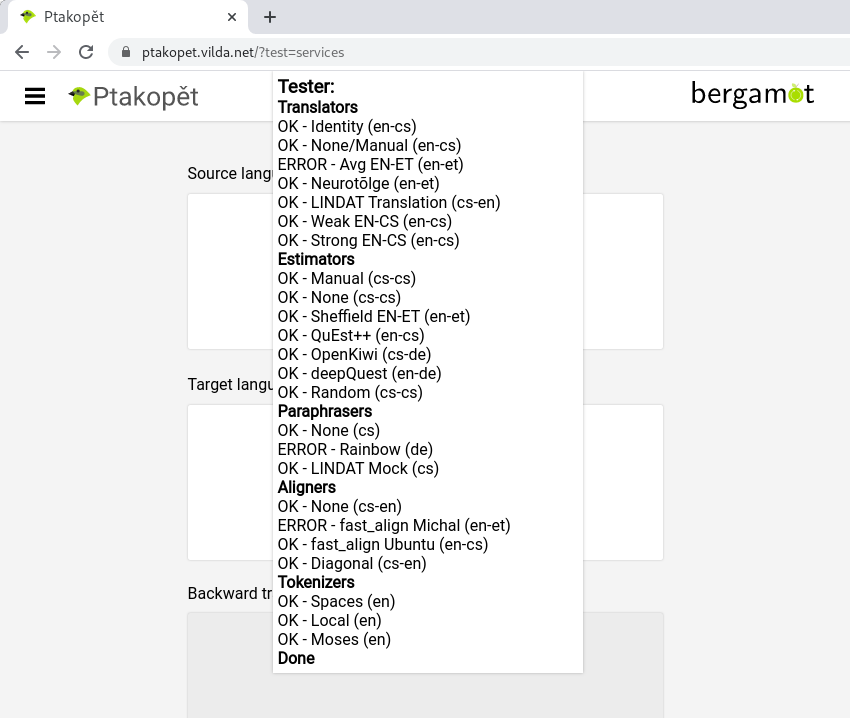
\includegraphics[width=\textwidth]{img/implementation/test_services.png}
    \caption{Results of testing of all \ptakopet{} backends. Three backends were down at the moment.}
    \label{fig:test_services}
\end{figure}

\subsubsection{Testing} \label{subsubsec:implementation_testing}

The \texttt{Tester} class contains two functions. The first one, \texttt{workload}, simulates the user's workflow by changing the source input field in some fixed interval. This was used for debugging memory leaks, such as the one which was present in the pilot study (\cref{subsubsec:experiment_leak}). It can be invoked by adding the \texttt{test=workload} URL GET parameter.

The other function is used for testing the availability of backends. Since \ptakopet{} encompasses many backends it is necessary to monitor their status. To get a summary of their availability add the \texttt{test=services} URL GET parameter. A white window will then appear at the top of the screen. The result is visible in \cref{fig:test_services}. This function sends requests to all available backends (even local ones) with a prepared text input and language settings. Usually the backend status (up or down) is manifested on a single call, so checking text and language variations is not necessary.


\subsubsection{Highlighting} 

Given a QE score from $0$ to $1$ the color is computed as in \cref{equation:implementation_color}. It is substracted from one, because QE of $1$ correspond to high confidence and we want to highlight bad scores. It is also scaled down by $\frac{1}{3}$ for the highlighting to not be too disruptive in the user interface. Technical details of highlighting are described in \cref{subsubsec:dev_doc:highlighting}.

\begin{equation}
        \text{color}(qe) = \text{RGBA}\big(1, 0, 0, \frac{1-qe}{3}\big)
    \label{equation:implementation_color}
\end{equation}

\subsubsection{Source complexity} \label{subsubsec:impl:source_complexity}

After the quality estimation and alignment is computed, every source word receives a possibly empty set of QE scores. This is because the alignment may map the source word to zero or more target words. Different aggregating functions can be chosen to get a single number, for example \textit{maximum}, \textit{minimum}, \textit{average} or \textit{weighted average (by position)}. Furthermore the default QE score has to be assigned to unaligned tokens. We found it reasonable to use the \textit{average} aggregating function as to consider all the provided scores. The score for unaligned tokens was set to $0.9$ to only slightly hint that something may be wrong.

\pagebreak
\section{Experiment definition} \label{sec:experiment_def}

An experiment can be defined in a single JSON file. The format, details and relevant tools used for generating experiment materials are described in detail in \cref{sec:dev_doc:experiment_def}.

In the experiment definition we need to specify the number of users, their user IDs and the queues. In this context we use the term ``baked queues'' for every user which is just pre-generated random sequence of stimuli and their configurations. This way it is decided prior to the experiment what stimuli configurations and in what order will a given users encounter them. Baked queues are described more in detail in \cref{subsec:experiment:technical_details}.

A stimuli is just a string containing a HTML code which gets pasted into the webpage. This is flexible enough to allow for both images and texts with highlights. Every stimuli can be also presented with a different configuration, such as a specific backend and set of modules enabled.


\section{Server backend}
\label{sec:server-backend}

The server backend's purpose is to make some of the MT related services (quality estimation, alignment, tokenization) available to the frontend. It is necessary, as most of these services are not publicly deployed, but is not the main focus of the \ptakopet{} project, nor of this thesis. Even though it was created to be portable in theory, it is not expected to be run on any other server than ours. It is written in Python~3.

To run the server (on \texttt{0.0.0.0:80}), launch the \texttt{server/run.sh} script. A common practice is to connect to a remote machine via SSH and launch the server. For that, there is a script \texttt{server/run\_nohup.sh}, which disregards kill signals on user logout.

\begin{figure}[ht]
    \centering
    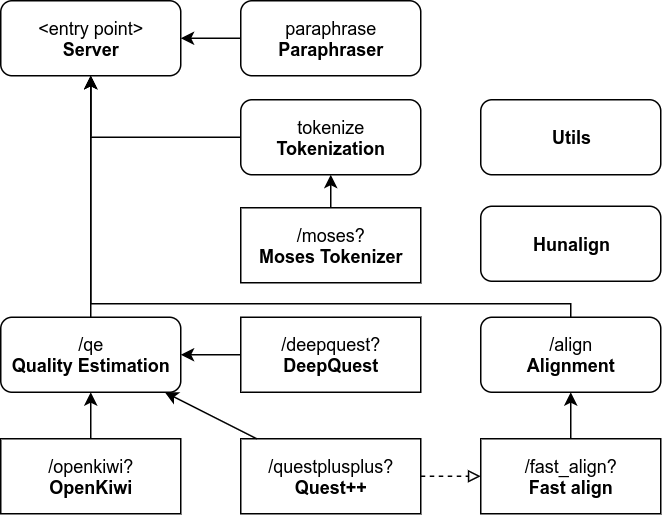
\includegraphics[width=0.8\textwidth]{img/implementation/backend.png}
    \caption{Object diagram of main components of the \ptakopet{} backend}
    \label{fig:backend_class}
\end{figure}

\subsection{Architecture and API}

The overall backend object architecture is shown in \cref{fig:backend_class}. The dashed line from QuEst++ to Fast align means that QuEst++ uses this alignment tool also as part of its pipeline. Both GET and POST methods are accepted. The server offers the following API calls. In \cref{lst:backend_examples_1} and \cref{lst:backend_examples_2}, we show example requests together with their responses. The sentence aligner Hunalign is not accessible publicly and is used only for internal purposes.


\begin{itemize}
    \item \texttt{qe/[openkiwi, deepquest, questplusplus]/?} - for word-level QE. \\
    Requires: \texttt{sourceLang} \texttt{targetLang}, \texttt{sourceText} and \texttt{targetText}.
    
    \item \texttt{align/[fast\_align]/?} - word alignment. \\
    Requires: \texttt{sourceLang} \texttt{targetLang}, \texttt{sourceText} and \texttt{targetText}.
    
    \item \texttt{tokenize/[moses]/?} - sentence tokenization. \\
    Requires: \texttt{text} and \texttt{lang}.
    
    \item \texttt{paraphrase/[mock]/?} - paraphrasing. \\
    Requires: \texttt{text} and \texttt{lang}.
\end{itemize}


\begin{lstlisting}[caption={Three examples of \ptakopet{} backend quality estimation, tokenization and alignment requests and responses}, label={lst:backend_examples_1}, escapeinside={\%*}{*)}, stringstyle=\ttfamily, showstringspaces=false]
qe/deepquest
    ?sourceLang=cs
    &targetLang=de
    &sourceText=%*Student gymnázia.*)
    &targetText=Ein Student der Gymnastik.
    
-> {"status": "OK", 
    "qe": [0.8, 0.5, 0.2, 0.5, 1.0]}

tokenize/moses
    ?text=(z.B. Tomaten, Karotten usw.)
    &lang=de
    
-> {"status": "OK",
    "tokenization": ["(", "z.B.", "Tomaten",
                     ",", "Karotten", "usw.", ")"]}
               
align/fast_align
    ?sourceLang=en
    &targetLang=de
    &sourceText=Click the mouse button.
    &targetText=Klicken Sie mit der Maustaste.
    
-> {"status": "OK",
    "alignment": "0-0 0-1 2-2 1-3 3-4 4-5"}
\end{lstlisting}
               
\begin{lstlisting}[caption={An example of \ptakopet{} backend paraphrase request and response}, label={lst:backend_examples_2}, escapeinside={\%*}{*)}, stringstyle=\ttfamily, showstringspaces=false]
paraphrase/mock
    ?lang=cs
    &text=%*Jsem student posledního ročníku gymnázia.*)
    
-> {"status": "OK",
    "de": %*"Poslední rok studuji gymnastiku.",*)
    "fr": %*"Jsem v posledním ročníku střední školy.",*)
    "ru": %*"Jsem ve čtvrťáku na gymnáziu.",*)
    "en": %*"Jsem ve čtvrťáku na gymnáziu."*)}
\end{lstlisting}


\subsection{Data and trained models}

\subsubsection{Word alignment}

Fast align is the only alignment model we deployed. It simply requires a bilingual sentence aligned corpus. We add the incoming language pairs to the data and run Fast align. For the corpora, we make use of Ubuntu localization files.\footnotehref{http://opus.nlpl.eu/Ubuntu-v14.10.php}{opus.nlpl.eu/Ubuntu-v14.10.php} We chose the IT domain, because data for the QE models are only in this domain. The server is distributed with the following language pairs: \texttt{cs-de}, \texttt{cs-en}, \texttt{cs-fr}, \texttt{en-de}, \texttt{en-es}, \texttt{en-et} and \texttt{en-fr}.

\subsubsection{Quality estimation}

The original feature extractor system in QuEst++ supports English$\rightarrow$Spanish quality estimation. We experimented with feeding it English$\rightarrow$Czech quality estimation data and expected that the ML part would disregard noisy or low information features caused by feeding the feature extractor unsupported language. We found that the performance regressed so considerably that we did not experiment further and focused on other QE systems.

Both DeepQuest (bRNN) and OpenKiwi (Predictor-Estimator) were trained on WMT 2017 English-German Word Level Quality Estimation dataset in the IT domain \citep{WMT17}. These trained models are downloaded automatically when running the backend install script. 
OpenKiwi, in general, proved to be faster, more robust and easier to use than DeepQuest. Because of this, the experiment was conducted with OpenKiwi quality estimation backend.

\subsubsection{Czech-German Quality Estimation Dataset} \label{subsec:cs_de_wmt}

For the experiment, we also needed to train a Czech$\rightarrow$German QE model. Since relevant Czech$\rightarrow$German training data for QE were not available, we synthesized them from English$\rightarrow$German data. We processed the WMT17 English-German data to obtain Czech$\rightarrow$German data by translating the source language sentences using LINDAT Translation \cite{popel-en-cs} from English to Czech. Given triplets (English, German, QE), we thus create triplets of (Czech, German, QE). An example of this can be seen in \cref{fig:tripel_qe_example}.

\begin{figure*}[ht]
    \centering
    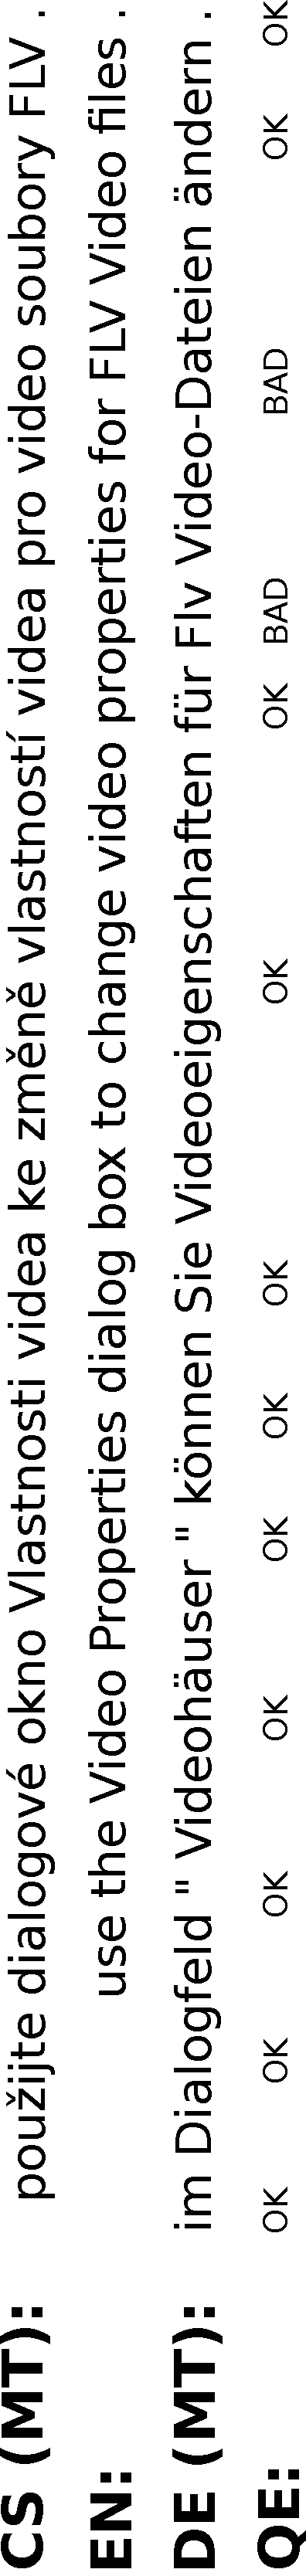
\includegraphics[height=\textwidth, angle=-90]{img/implementation/qe_example_pdfa1a.pdf}
    \caption{\label{fig:tripel_qe_example} Quality estimation tags for tokens and gaps on German sentence translated from English (from WMT19 quality estimation shared task) together with synthetic Czech source (translated from English). MT systems are independent.}
\end{figure*}

To make sure the data did not lose quality, we performed the following experiment: We manually annotated 30 Czech-German and 20 English-German sentences for word-level quality estimation, in the same format as the original English-German dataset, i.e., labeling German words with OK/BAD labels given the source sentence. The original English-German annotation served as the golden standard. Our annotation for English-German was created independently of it and it served as a benchmark for our agreement with the original. 

\begin{table}[ht]
    \centering
    \begin{tabular}{| l l |}
        \hline
        \multicolumn{2}{|c|}{All}\\
        \hline
        TP=74.57\%& FP=2.68\%\\
        FN=12.98\%& TN=9.76\%\\
        \hline
        \multicolumn{2}{|c|}{Czech$\rightarrow$German}\\
        \hline
        TP=77.58\%& FP=3.68\%\\
        FN=11.03\%& TN=7.71\%\\
        \hline
        \multicolumn{2}{|c|}{English$\rightarrow$German}\\
        \hline
        TP=69.81\%& FP=1.11\%\\
        FN=16.07\%& TN=13.02\%\\
        \hline
    \end{tabular}
    \caption{\label{tab:manual_qe_annotation}Confusion matrix for word-level quality estimation annotations of Czech-German and English-German.}
\end{table}

\cref{tab:manual_qe_annotation} shows the confusion matrices of our annotations compared to the golden standard. The distributions for both language pairs are similar. The sample is very small and the sets of underlying sentences (20 English and 30 Czech) had to be different because the annotation was carried out by a single person, but the results nevertheless indicate that this transfer of QE data by machine-translating the source is viable. The similarity of confusion scores can mean one of the following. Either the German sentence itself was representative enough for the annotator to produce classes with similar distributions, or that both the English and the Czech sentences provided the same level information. In both cases, the pairs (EN, DE) and (CS, DE) seem equally usable, which means that we should be able to train a similarly good quality estimation model based on the synthetic Czech source.